\documentclass[12pt]{article}

% Package
\usepackage{graphicx} % Add images package
\usepackage{listings} % Add code file package

% Document settings
\graphicspath{{../images}}
\setlength{\parindent}{0pt}

% Documentation title
\title{Sommatore a 3 input (v1)}
\author{Stefano Scarcelli \& Michele De Fusco}
\date{01 Dic 2023}


% Document
\begin{document}
% Cover
\maketitle
\newpage

% Indice
\tableofcontents
\newpage

% Document body

\section{Analisi progettuale}
    \subsection{Analisi preliminare}
        L'obbiettivo è quello di costruire un circuito in grado di sommare 3 numeri a \textit{n-bit} (\textit{2's complements}) e restituirne il risultato. Sia gli input che gli output devono essere sincronizzati tramite l'uso di registri.

        L'idea di base è quella di usare due \textbf{Ripple carry} \textit{parametrici} in cascata tra di loro per eseguire il calcolo desiderato $A+B+C=R$.
    
    \subsection{Struttura del progetto}
        L'idea alla base dell'implementazione è quella di inserire in pipeline i due moduli \textbf{sommatori} per eseguire prima la somma $A+B$ e successivamente $(A+B)+C$.

        Questa implementazione porta all'inserimento di (in totale) di 6 \textbf{registri}, 2 in ingresso ad ogni adder, uno in aggiunta all'input $C$ per salvare il risultato per la seconda operazione di somma e uno in uscita per salvare il risultato dell'operazione complessiva (richiesto dalle specifiche del progetto).

        Il primo ritardo per riceve un risultato coerente è di 3 colpi di clock mentre il delay per ricevere i risultati successivi al primo è di solo 1 colpo di clock.

\section{Implementazione}
    L'implementazione si basa sulla definizione di una struttura gerarchica di componenti, partendo dalla definizione comportamentale dei componenti elementari (\textbf{Adder n-bit} e \textbf{Register n-bit}) per poi andare a comporre (tramite 2 livelli di astrazione, \textbf{Synched adder} e in fine l'elemento principale \textbf{Three adder (main)}) la struttura del progetto.

    \subsection{Adder n-bit}
        L'implementazione dell'\textbf{Adder n-bit} segue la descrizione comportamentale tramite \textbf{Ripple carry} parametrico usando i segnali \textit{propagate} ($P$) e \textit{generate} ($G$).

        \subsubsection{Codice VHDL}
            \lstinputlisting[language=vhdl, basicstyle=\footnotesize]{../../../Vivado_project_v1/Vivado_project_v1.srcs/sources_1/new/Adder.vhd}
            
        \subsubsection{Sintesi}
            \begin{figure}[ht]
                \centering
                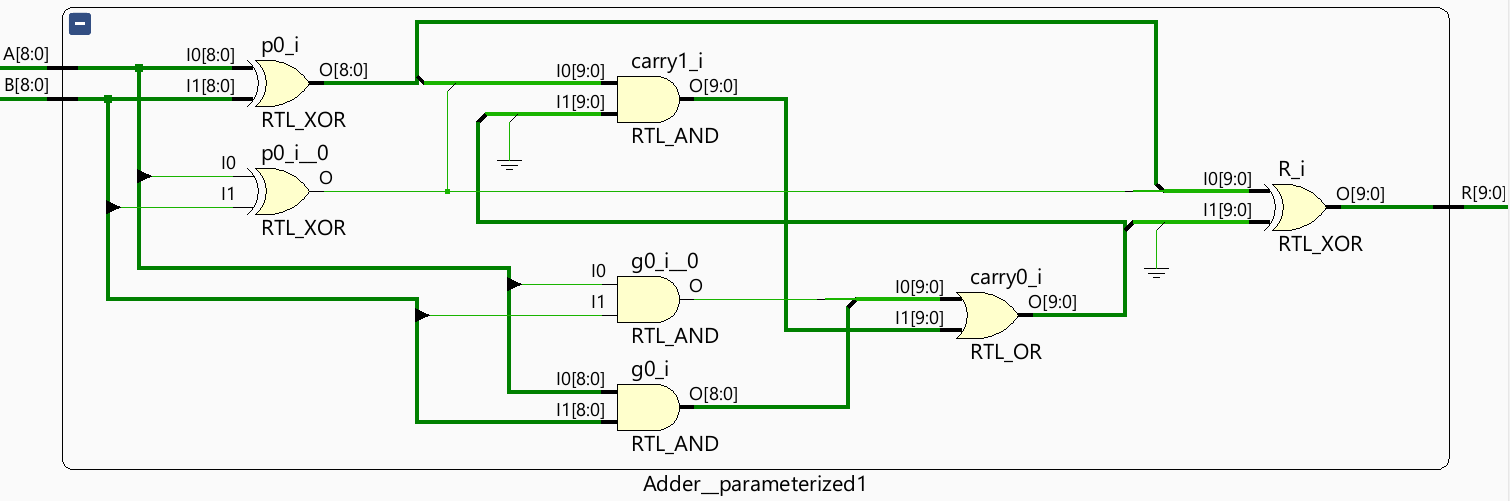
\includegraphics[scale=0.5]{Adder.png}
                \caption{Circuito di \textbf{Adder}.}
            \end{figure}

    \subsection{Register n-bit}
        L'implementazione dell'\textbf{Register n-bit} segue la descrizione comportamentale classica con memorizzazione a \textit{fronti di salita}.
        
        Il \textbf{registro} implementa in più un segnale di \textit{clear} (asincrono) attivo alto.

        \subsubsection{Codice VHDL}
           \lstinputlisting[language=vhdl, basicstyle=\footnotesize]{../../../Vivado_project_v1/Vivado_project_v1.srcs/sources_1/new/Register_n.vhd}
            
        \subsubsection{Sintesi}
            \begin{figure}[ht]
                \centering
                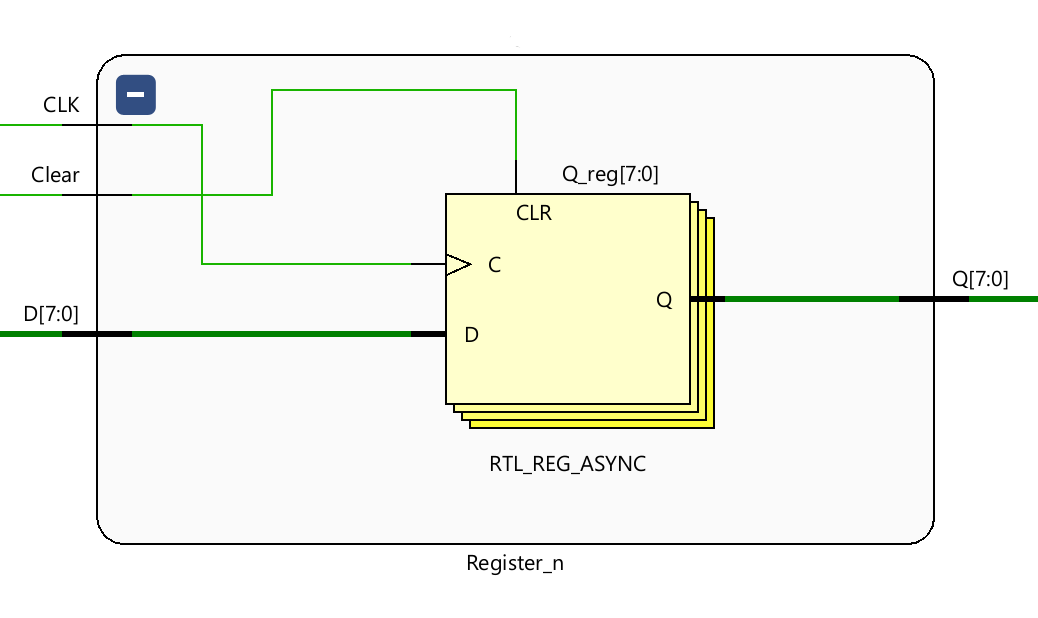
\includegraphics[scale=0.45]{Register.png}
                \caption{\textbf{Registro} a 8bit.}
            \end{figure}

    \subsection{Synched adder}
        Questo è un componente intermedio che abbiamo impostato per poi costruire il circuito completo.

        Consiste in un \textbf{Adder n-bit} con 2 \textbf{registri} collocati agli input di esso.

        \subsubsection{Codice VHDL}
            \lstinputlisting[language=vhdl, basicstyle=\footnotesize]{../../../Vivado_project_v1/Vivado_project_v1.srcs/sources_1/new/Synched_adder.vhd}
        
        \subsubsection{Sintesi}
            \begin{figure}[ht]
                \centering
                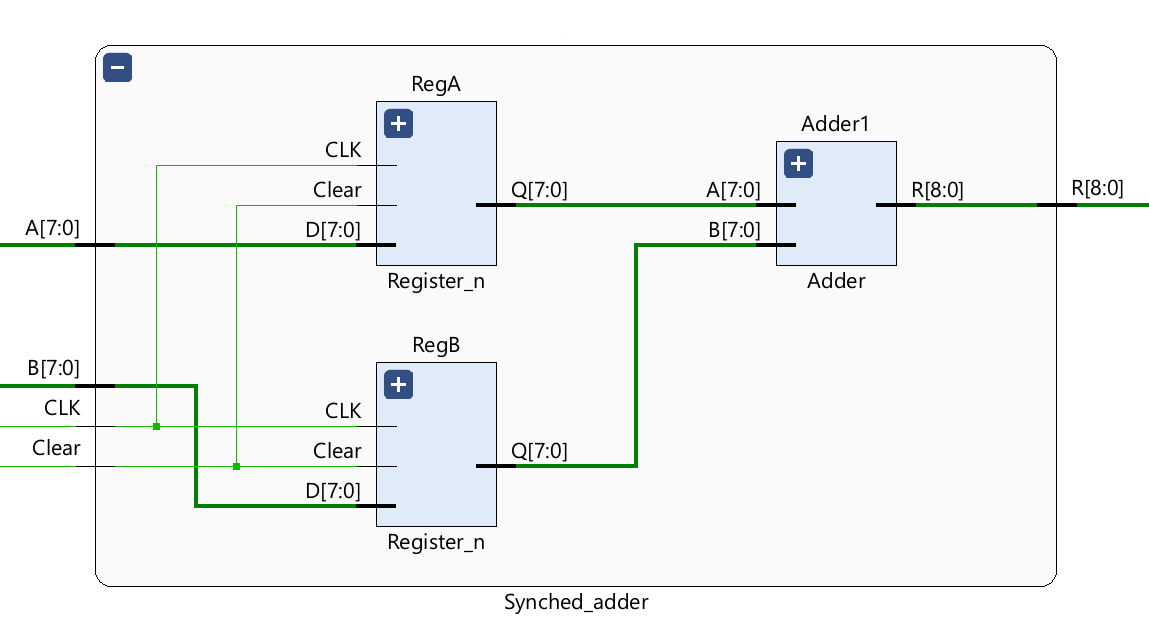
\includegraphics[scale=0.75]{Synched_adder.png}
                \caption{Circuito del \textbf{Synched adder}.}
            \end{figure}

    \subsection{Three adder (main)}
        Il circuito finale comprende invece l'uso di 2 \textbf{Synched adder} e 2 \textbf{registri} aggiuntivi, uno collocato tra l'input $C$ del circuito e il secondo ingresso del secondo \textbf{Synched adder} (usato come buffer per salvare il valore di $C$ nella pipeline) e un'altro tra il risultato dell'operazione e l'output del circuito (come richiesto dalle specifiche del progetto).

        \subsubsection{Codice VHDL}
            \lstinputlisting[language=vhdl, basicstyle=\footnotesize]{../../../Vivado_project_v1/Vivado_project_v1.srcs/sources_1/new/Three_Adder.vhd}
        \newpage
        
        \subsubsection{Sintesi}
            \begin{figure}[ht]
                \centering
                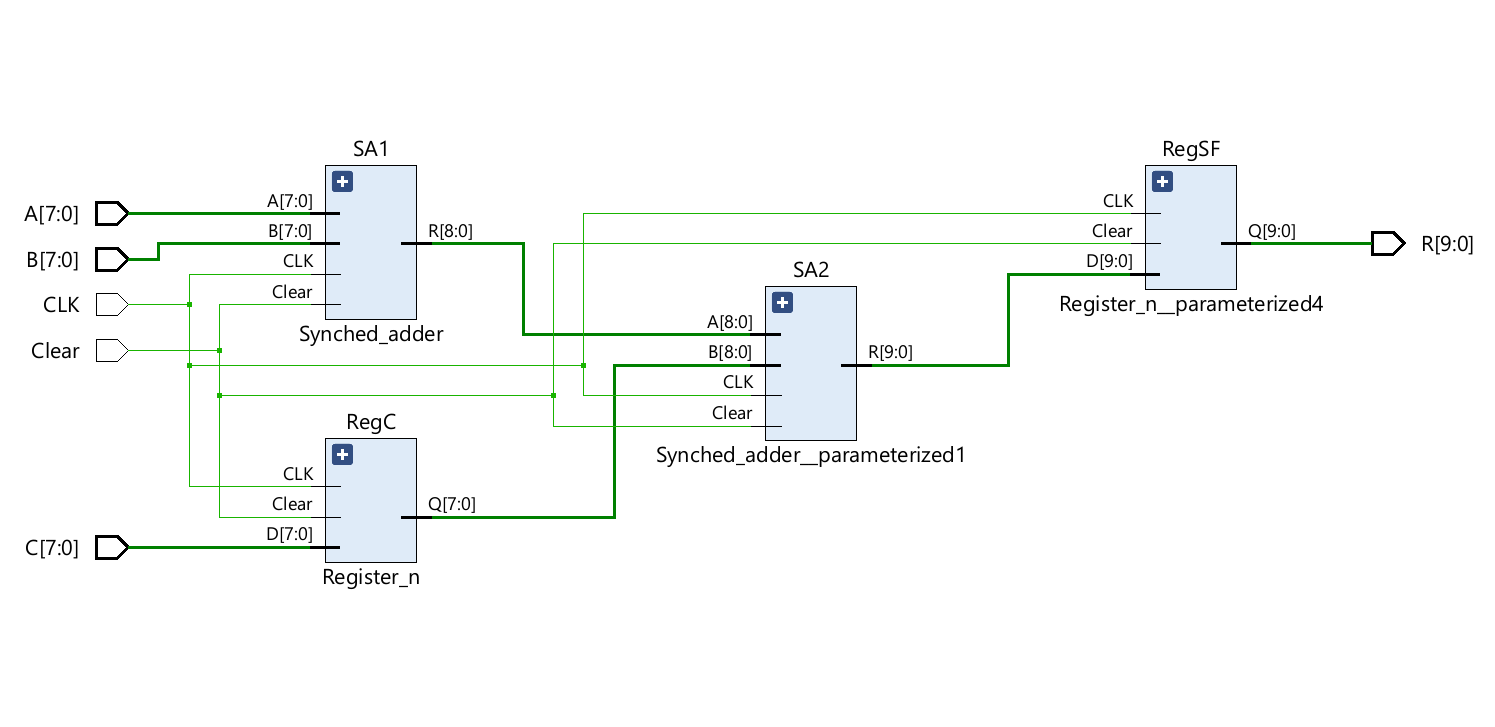
\includegraphics[scale=0.55]{main.png}
                \caption{Circuito principale.}
            \end{figure}

    \subsection{Time constrain}
        In più abbiamo aggiunto un \textit{time constrain} sul segnale di clock con un periodo di \textbf{5ns}.

        \begin{lstlisting}[basicstyle=\footnotesize]
            create_clock -period 5.000 -name main_clock
            -waveform {0.000 2.500} [get_nets CLK]
        \end{lstlisting}

        \subsubsection{Analisi del Time constrain}
            Con l'implementazione del codice abbiamo verificato (\textit{Timing summary routed}) che il \textbf{Time constrain} fosse valido, valutando di aver inserito un periodo di clock di superiore rispetto al minimo tollerabile dal circuito di \textbf{1.958ns}.
        
\section{Testing}
    Per il test abbiamo optato ad una analisi parziale eseguendo somme di numeri che potessero stressare al massimo i componenti circuitali per verificarne il corretto funzionamento.

    \subsection{Codice test test-bench}
        \lstinputlisting[language=VHDL, basicstyle=\footnotesize]{../../../Vivado_project_v1/Vivado_project_v1.srcs/sim_1/new/Sim_Add.vhd}

    \subsection{Risultati}
        I risultati della simulazione post implementativa confermano il funzionamento del circuito come previsto.

        \begin{figure}[ht]
            \centering
            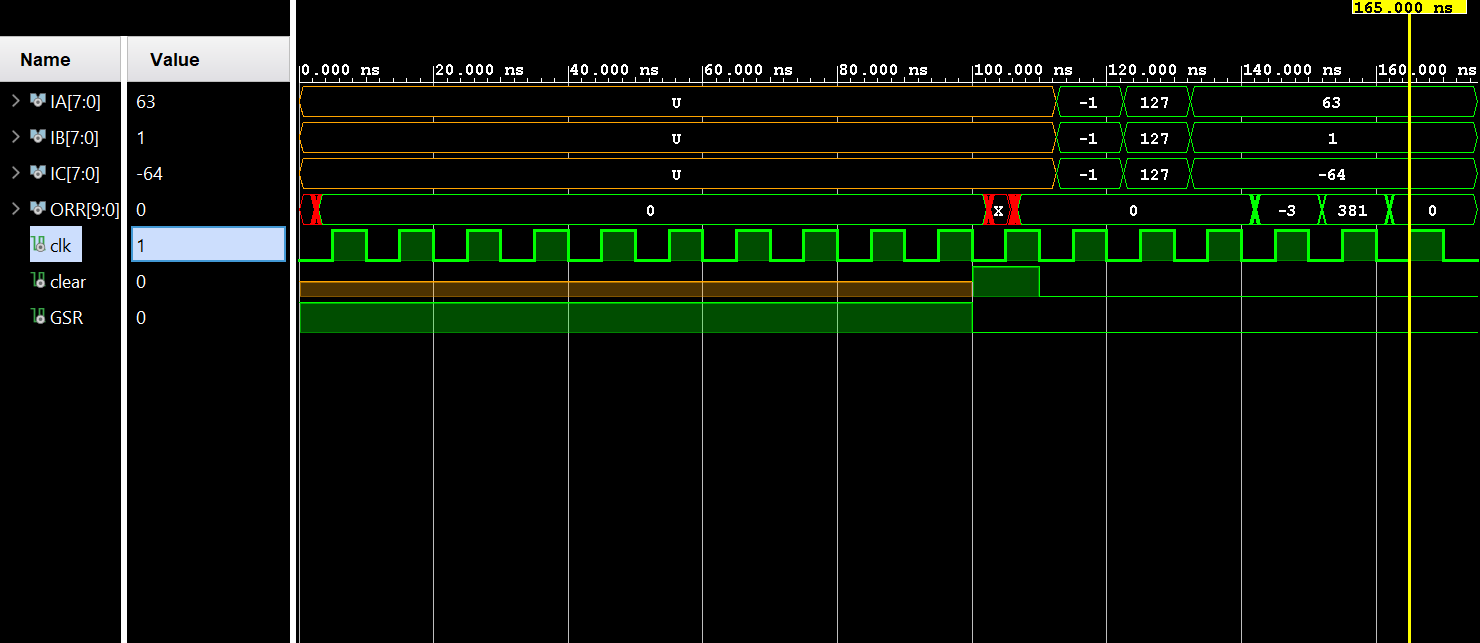
\includegraphics[scale=0.55]{Test.png}
            \caption{Grafico temporale simulazione post implementazione.}
        \end{figure}

\end{document}